\documentclass[11pt]{article}

% ============================================================
%  The Vowel Space Model -- A Didactic Introduction
%  Companion documentation to arXiv:2111.00868 (F. Berthommier)
%  Free toolchain only: article + amsmath + newtx + hyperref.
%  Build:  pdflatex tutorial   (twice, for the cross-references)
% ============================================================

\usepackage[letterpaper, total={6.9in,9.2in}]{geometry}
\usepackage[utf8]{inputenc}
\usepackage[T1]{fontenc}
\usepackage{amsmath, amssymb, bm}
\usepackage{amsthm}
\usepackage{tipa}
\usepackage[round]{natbib}
\usepackage{newtxtext, newtxmath}
\usepackage{graphicx}
\usepackage{booktabs}
\usepackage{enumitem}
\usepackage[colorlinks=true, linkcolor=blue!50!black, citecolor=blue!50!black,
            urlcolor=blue!50!black]{hyperref}

% --- pointers -----------------------------------------------------------
\newcommand{\arxivpaper}{\href{https://arxiv.org/abs/2111.00868}{arXiv:2111.00868}}
\newcommand{\repobase}{https://github.com/FBerthommier/vocalic-spaces}
\newcommand{\repo}[1]{\href{\repobase/#1}{\texttt{#1}}}
\newcommand{\code}[1]{\texttt{#1}}

% --- didactic environments ----------------------------------------------
\theoremstyle{definition}
\newtheorem{keyidea}{Key idea}
\newtheorem{exercise}{Exercise}
\theoremstyle{remark}
\newtheorem{remark}{Remark}

\newcommand{\Fone}{F_1}
\newcommand{\Ftwo}{F_2}

\title{\bfseries The Vowel Space Model:\\[2pt] A Didactic Introduction}

\author{Fr\'ed\'eric Berthommier\\
\small Univ. Grenoble Alpes, CNRS, Grenoble INP, GIPSA-lab, Grenoble, France}
\date{\small Companion tutorial to the research article \arxivpaper{}
(\emph{A mathematical model of the vowel space}).\\
Code, data and multimedia: \repo{} (this repository).}

\begin{document}
\maketitle

\begin{abstract}
\noindent
This tutorial develops, step by step and with worked numerical examples,
the theoretical content of the research article \emph{A mathematical
model of the vowel space} (\arxivpaper{}).  It is aimed at graduate
students and researchers in speech science, acoustics or signal
processing who want to understand \emph{why} a two-variable generative
model can fill the vowel space ($\Fone,\Ftwo$) and \emph{how} the
coordination function links articulatory models to it.  Every construction
is illustrated by the validated Python code of this repository, so each
section can be reproduced by running one script.  The research article
itself is available on arXiv; it is not part of this repository.
\end{abstract}

\tableofcontents

% ======================================================================
\section{The problem: a many-to-one articulatory--acoustic map}
% ======================================================================

A vowel sound is characterized, to first order, by its two lowest
resonances, the formants $\Fone$ and $\Ftwo$.  These resonances are
determined by the \emph{area function} $A(x)$: the cross-sectional area
of the vocal tract as a function of the distance $x$ from the glottis
($x=0$) to the lips ($x=L$, with $L\approx 17.5$\,cm for an adult male).
The map $A(x)\mapsto(\Fone,\Ftwo)$ is
\begin{itemize}[nosep]
\item \textbf{many-to-one}: very different tract shapes give nearly the
      same two formants (a constrictions at the front or at the back of
      the tract can act alike on $\Fone$);
\item \textbf{nonlinear}: doubling a constriction area does not double
      anything in $(\Fone,\Ftwo)$.
\end{itemize}
This is why acoustic-to-articulatory inversion has no reliable general
solution.  The article proposes a construct that restores a
\emph{bijection}: a two-dimensional family of area functions, indexed by
two latent variables, whose image in the $(\Fone,\Ftwo)$ plane is the
vowel triangle, with a one-to-one correspondence between the family and
its acoustic image.

\begin{keyidea}
Instead of fighting the many-to-one relation on real shapes, build the
\emph{simplest possible} parametric family of shapes for which the map to
$(\Fone,\Ftwo)$ is provably one-to-one, then transfer this construction
to human-like articulatory models through a single formula, the
\emph{coordination function}.
\end{keyidea}

\paragraph{Notation.}  Vectors are bold ($\bm{v}$); $A(x,\theta)$ denotes
an area function of the family parameterized by the cycle angle $\theta$;
$\rho\in[0,1]$ is a radial amplitude; $\bm{1}$ is the constant vector
equal to~1 (the neutral tube of unit area).

% ======================================================================
\section{The physical anchor: the Schroeder--Ehrenfest relation}
% ======================================================================

Linearize the acoustics around the neutral tube $\bm{1}$.  Writing the
area function as a small perturbation
$A(x)=1+\epsilon\,a(x)$, the eigenfrequencies of the closed--open tube
shift according to a Rayleigh quotient.  Using Ehrenfest's analogy
$\delta f_i/f_i=\delta E_i/E_i$ between the acoustic modes and a
quantum system, \citet{Schroeder1967} showed that the first-order
frequency shifts are governed by the \emph{odd cosine Fourier
coefficients} of the perturbation:
\begin{equation}
\frac{\delta f_i}{f_i}\;=\;-\frac{1}{2}\,a_i,
\qquad
a_1=\frac{2}{n}\sum_{k=1}^{n}A_k\cos\Big(\tfrac{\pi(k-\frac12)}{n}\Big),\quad
a_2=\frac{2}{n}\sum_{k=1}^{n}A_k\cos\Big(\tfrac{3\pi(k-\frac12)}{n}\Big),
\label{eq:SE}
\end{equation}
where $a_1$ weights the mode shape $v_1=\cos(\pi x/L)$ and $a_2$ the mode
shape $v_2=\cos(3\pi x/L)$.  Intuition: the first mode has an antinode at
the lips and a node at mid-tube, so a front narrowing (large $v_1$
positive region) lowers $\Fone$; the second mode changes sign twice and
is mostly sensitive to the middle third of the tract, controlling
$\Ftwo$.

\begin{remark}
Relation~\eqref{eq:SE} is \emph{exact at first order} around the neutral
tube only.  The whole article can be read as the study of how far this
linear rule survives (i) far from the neutral tube, (ii) after a
rectification of the area function, and (iii) in articulated models.  The
answer, derived in \S\ref{sec:bias}, is: remarkably far, up to one
quadratic term on $\Fone$.
\end{remark}

% ======================================================================
\section{The three-phase mixing function}
% ======================================================================

\subsection{From the Gibbs triangle to a cycle}

In chemistry, a ternary mixture of components $(\bm{i},\bm{j},\bm{k})$
with proportions summing to one is drawn inside a triangle (the Gibbs
triangle); the mixture is the convex combination
$p=\alpha\bm{i}+\beta\bm{j}+\gamma\bm{k}$ with
$\alpha+\beta+\gamma=1$.  The article uses a different slice of the same
construction: fix the \emph{sum} of the three weights and let them
oscillate, which produces a \emph{closed cycle} through the three
components instead of a filled triangle:
\begin{equation}
\bm{P}(\theta)=\frac{1}{3}\,(\bm{i}+\bm{j}+\bm{k})
+\frac{2}{3}\Big(\bm{i}\cos\big(\theta-\tfrac{\pi}{3}\big)
+\bm{j}\cos(\theta-\pi)
+\bm{k}\cos\big(\theta-\tfrac{5\pi}{3}\big)\Big).
\label{eq:mixing}
\end{equation}
Each component is visited at its own phase,
$\bm{P}(\tfrac{\pi}{3})=\bm{i}$, $\bm{P}(\pi)=\bm{j}$,
$\bm{P}(\tfrac{5\pi}{3})=\bm{k}$, and the mean over the cycle is the
neutral point $\bm{\Omega}=\frac13(\bm{i}+\bm{j}+\bm{k})$.  The acoustic
space is a triangle of extreme vowels \textipa{[u,\,a,\,i]} with the
neutral vowel \textipa{[@]} at its center; the shape space is a circle
through the three seed shapes, with the neutral tube at its center.  This
triangle$\,\leftrightarrow\,$circle pairing is the geometric core of the
model.

\subsection{The seed vectors \texorpdfstring{$\{\bm{i},\bm{j},\bm{k}\}$}{\{i,j,k\}}}

For the \emph{generic model}, the seeds are the simplest vector
functions that can push $\Fone$ and $\Ftwo$ to their extremes through
relation~\eqref{eq:SE}:
\begin{equation}
\bm{i}=\bm{1}+\bm{v_1}+\bm{v_2},\qquad
\bm{j}=\bm{1}-2\,\bm{v_1},\qquad
\bm{k}=\bm{1}+\bm{v_1}-\bm{v_2},
\label{eq:seeds}
\end{equation}
with $\bm{v_1}=\cos(\pi x/L)$ and $\bm{v_2}=\cos(3\pi x/L)$.
They satisfy $\bm{\Omega}=\frac13(\bm{i}+\bm{j}+\bm{k})=\bm{1}$ (the
neutral tube).  Expanding~\eqref{eq:mixing} with these seeds gives the
\emph{concise vowel equation}:
\begin{equation}
\bm{P}(\theta)=\bm{1}+a_1(\theta)\,\bm{v_1}+a_2(\theta)\,\bm{v_2},
\qquad
a_1(\theta)=2\cos\theta,\quad
a_2(\theta)=\tfrac{4}{3}\sin\tfrac{\pi}{3}\,\sin\theta .
\label{eq:Ptheta}
\end{equation}
Thus the two mixing coordinates are nothing but the two
Schroeder--Ehrenfest coefficients: \emph{the latent variables of the
model are the physically meaningful ones}.

\begin{exercise}
Show from~\eqref{eq:mixing} that
$\bm{P}(\theta+\pi)=2\bm{\Omega}-\bm{P}(\theta)$ (point symmetry about
$\bm{\Omega}$).  Deduce that the coefficients of the vowels
\textipa{[E, 1, O]} are the negatives of those of
\textipa{[u, a, i]}: $a_i(\theta+\pi)=-a_i(\theta)$.  This
\emph{antisymmetry} halves the number of seed shapes to specify.
\end{exercise}

% ======================================================================
\section{The generic model and its eight vowels}
% ======================================================================

Area functions must be positive; the raw mixture $\bm{P}(\theta)$ is
not.  A single explicit nonlinearity is introduced, the \emph{soft
rectifier}
\begin{equation}
\mathrm{expif}(y)=\begin{cases}e^{\,y-1}, & y<1\\ y, & y\ge 1\end{cases}
\qquad\text{(\code{expif} in \code{vsmodel/models.py}),}
\label{eq:expif}
\end{equation}
which is $C^1$ at $y=1$ and equal to the identity above it.  The generic
model is then
\begin{equation}
A(x,\theta)=\mathrm{expif}\Big(1+a_1(\theta)\cos\frac{\pi x}{L}
+a_2(\theta)\cos\frac{3\pi x}{L}\Big),
\label{eq:generic}
\end{equation}
with $L=17.5$\,cm as the only static parameter and
$\theta\in[0,2\pi)$ as the single control.  The eight cardinal vowels
correspond to eight phases, i.e.\ eight pairs $(a_1,a_2)$:

\begin{table}[h]
\centering
\small
\begin{tabular}{lcccccccc}
\toprule
vowel & \textipa{1} & \textipa{u} & \textipa{o} & \textipa{O} & \textipa{a}
       & \textipa{E} & \textipa{e} & \textipa{i} \\
\midrule
$\theta/\pi$ & $0$ & $1/3$ & $1/2$ & $2/3$ & $1$ & $4/3$ & $3/2$ & $5/3$ \\
$(a_1,a_2)$ & $(2,0)$ & $(1,1)$ & $(0,\alpha)$ & $(-1,1)$ & $(-2,0)$
            & $(-1,-1)$ & $(0,-\alpha)$ & $(1,-1)$ \\
$\Fone$ (Hz) & 188 & 259 & 377 & 576 & 886 & 586 & 386 & 267 \\
$\Ftwo$ (Hz) & 1665 & 984 & 848 & 953 & 1538 & 1961 & 2182 & 2124 \\
\bottomrule
\end{tabular}
\caption{The eight cardinal vowels of the generic model
($\rho=1$, $L=17.5$\,cm), with formants computed by the validated Python
TLM (\code{scripts/simu\_gen.py}; values reproduce the article within
1\,Hz).  $\alpha=\frac43\sin\frac{\pi}{3}$.  Extrema: $\min\Fone$
(\textipa{1}), $\max\Fone$ (\textipa{a}), $\min\Ftwo$ (\textipa{o}),
$\max\Ftwo$ (\textipa{e}) fall exactly on the four expected vowels.}
\label{tab:vowels}
\end{table}

Sampling $A(x,\theta)$ into $n\ge100$ tubelets and feeding it to the
transmission-line model (TLM) of \citet{BadinFant1984} yields the vowel
loop of Fig.~\ref{fig:loop}: despite the rectification
nonlinearity~\eqref{eq:expif}, the circle $(a_1,a_2)$ is mapped to a
rounded \emph{triangle} whose corners are the extreme vowels --- the
acoustic vowel triangle emerges from a circular control parameter.

\begin{figure}[t]
\centering
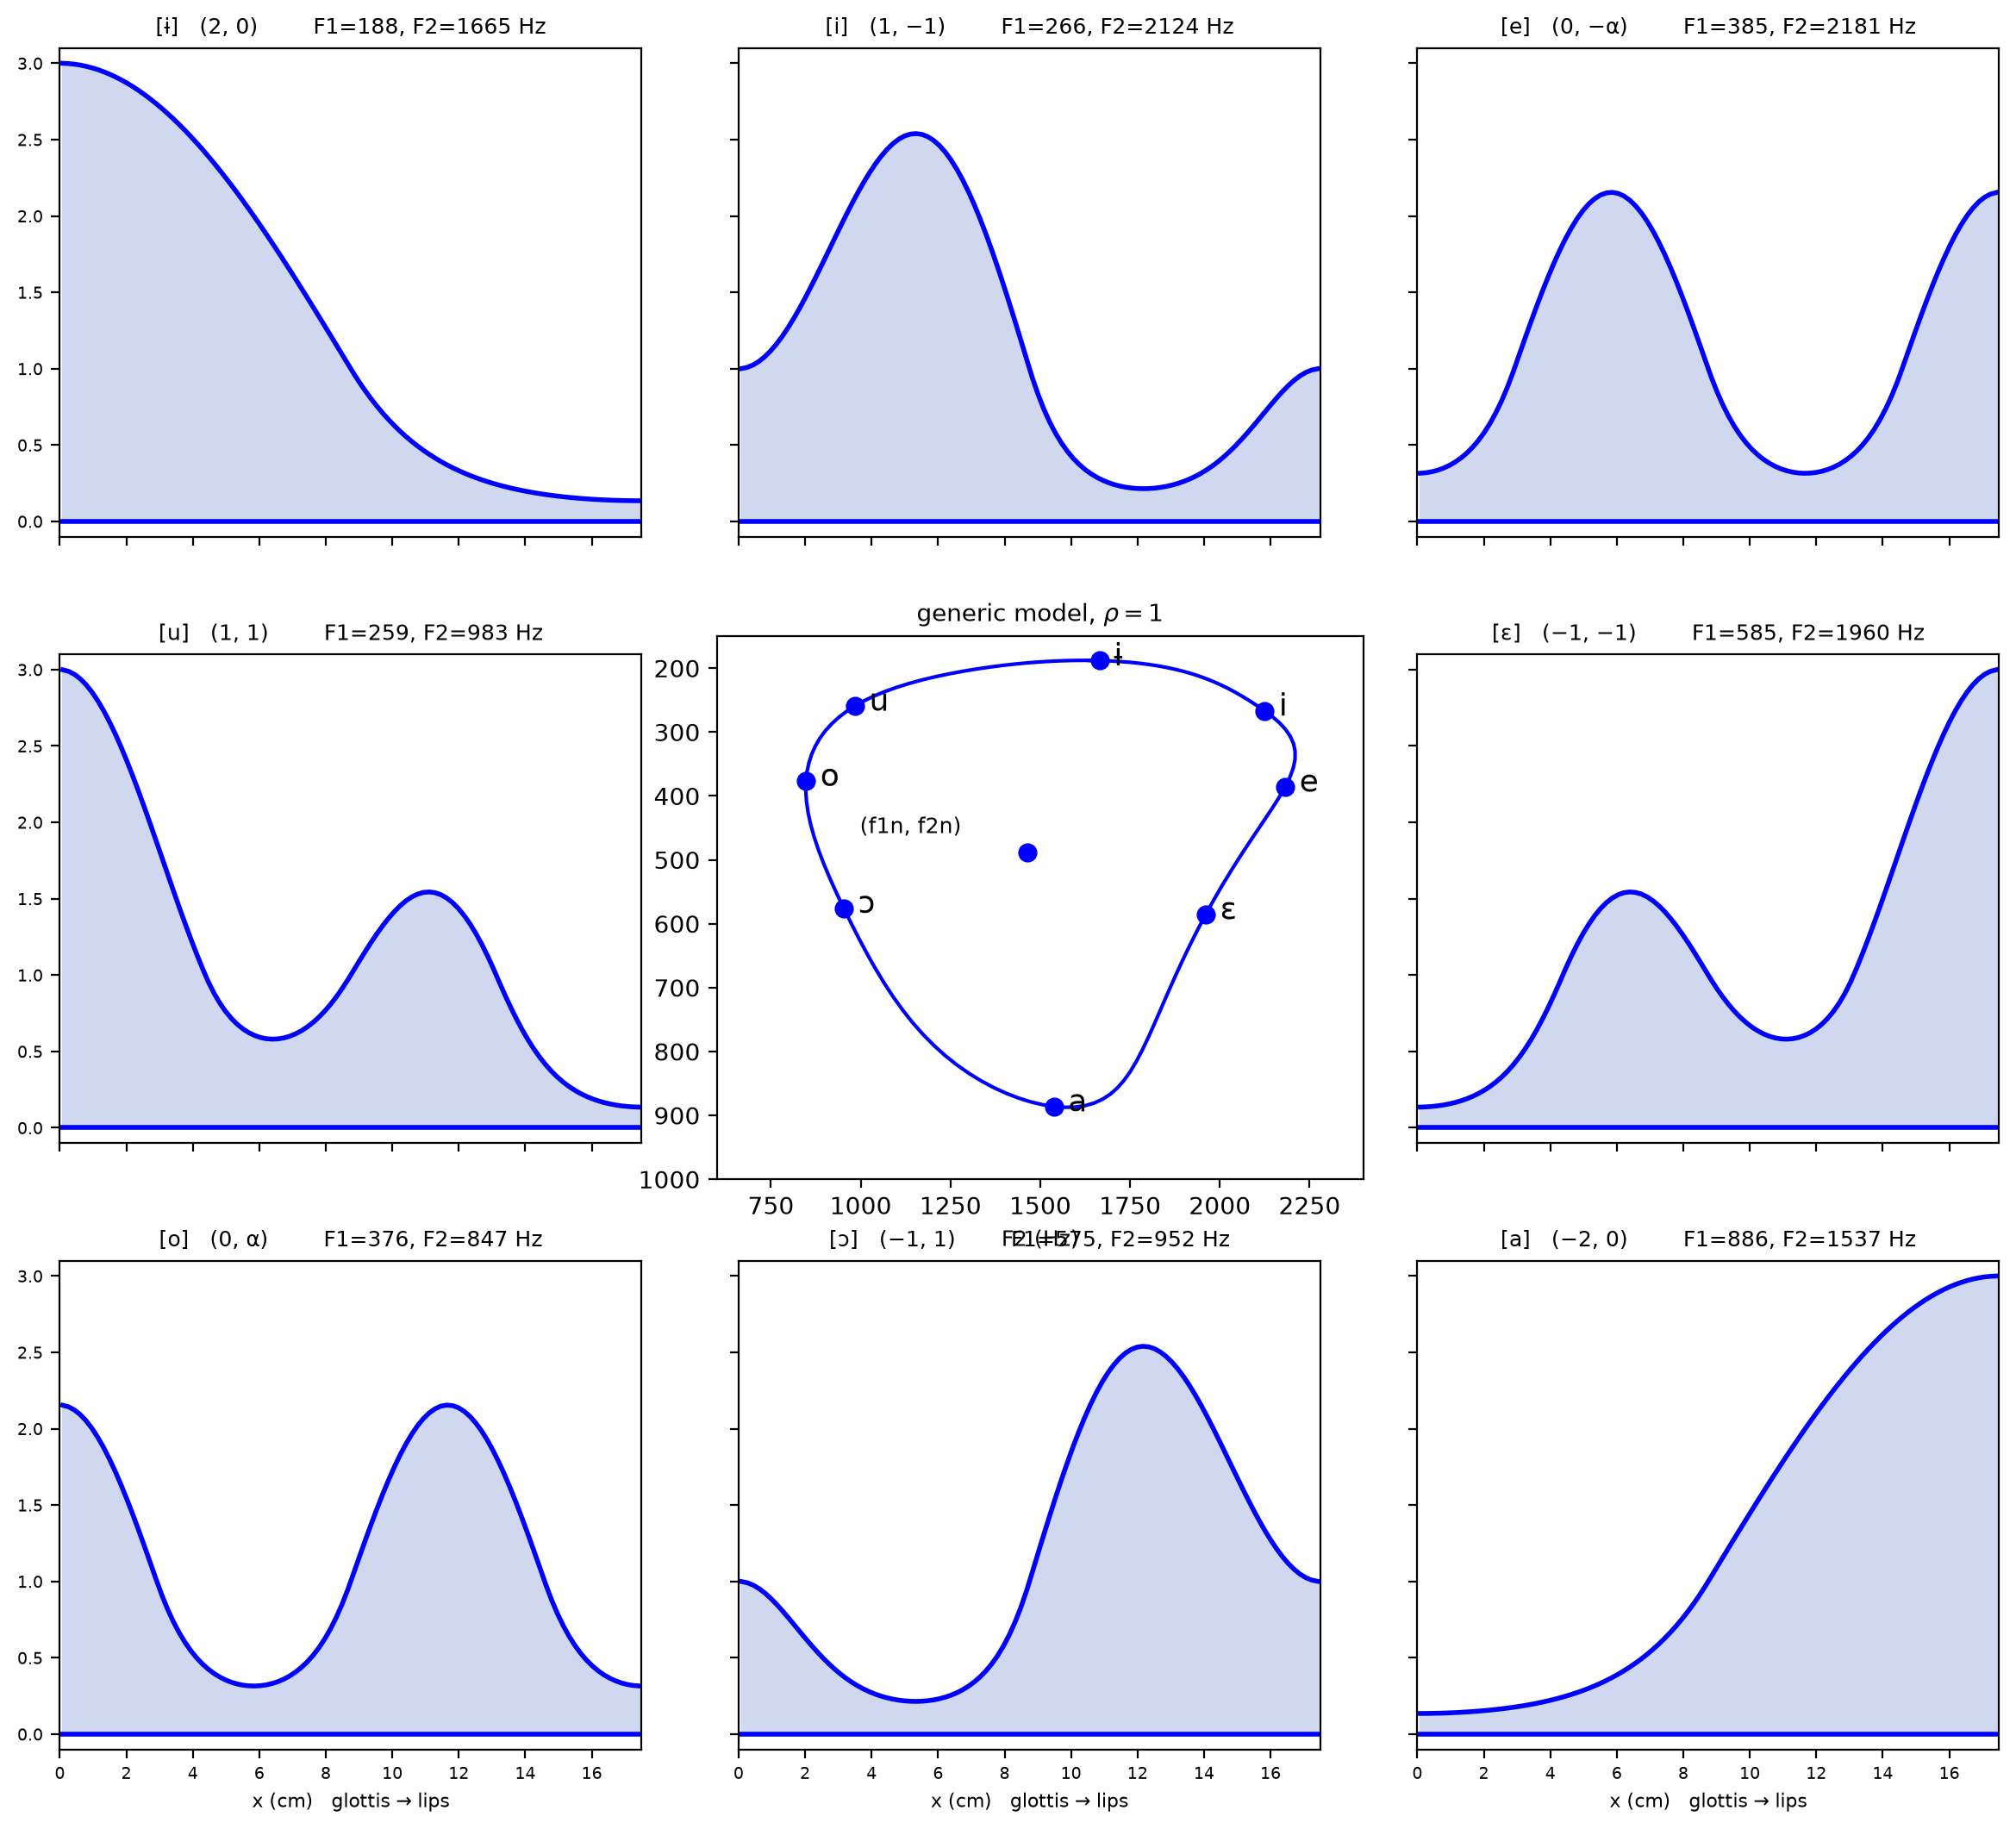
\includegraphics[width=0.62\textwidth]{../figures/Figure1.png}
\caption{Vowel space of the generic model and the eight area functions
(pairs $(a_1,a_2)$), reproduced by \code{scripts/fig1\_generic.py}.  The
same construction drives the multimedia files Mm.~1--2 of the article
(\code{multimedia/generated/MM1.wav}, \code{MM2.gif}).}
\label{fig:loop}
\end{figure}

\begin{exercise}
(\code{scripts/simu\_gen.py --quick})  Check that the neutral tube
($\rho=0$) gives $(\Fone,\Ftwo)=(488,1464)$\,Hz and that scaling both
coefficients by $\rho\in(0,1]$ sweeps a homothetic copy of the loop ---
the domain is filled, not just its boundary.
\end{exercise}

\begin{remark}[Why $\bm{n\ge100}$ tubelets?]
The sampled staircase approximation of $A(x)$ introduces small shifts of
the resonances; with $n=100$ they stay below $\sim$1\,Hz for
$(\Fone,\Ftwo)$, far below the just-noticeable difference.  The article's
results do not depend on the particular TLM implementation, only on
$n$ being large.
\end{remark}

% ======================================================================
\section{The coordination function}
\label{sec:coordination}
% ======================================================================

Equation~\eqref{eq:Ptheta} is a special case of a \emph{polar}
representation.  For \emph{any} vector parameter
$\bm{p}$ of an articulatory model (section areas, constriction position,
tract length, Maeda-style parameters\ldots), define the cycle
\begin{equation}
\bm{P}(\rho,\theta)=\bm{\Omega}+\rho\,\bm{\Psi_1}\cos(\bm{\Psi_2}-\theta),
\label{eq:coord}
\end{equation}
where the three dual vectors are obtained from the seed values
$\{\bm{i},\bm{j},\bm{k}\}$ of the parameter (its values on the three
extreme vowels) by
\begin{equation}
\bm{\Omega}=\tfrac13(\bm{i}+\bm{j}+\bm{k}),\qquad
\bm{\Psi_2}=\arctan\frac{(\bm{i}-\bm{k})\sin\frac{\pi}{3}}
{\frac12(\bm{i}+\bm{k})-\bm{j}},
\label{eq:ijk2psi}
\end{equation}
and $\Psi_{1,h}=(h-\Omega)/\cos(\Psi_2-\theta_h)$ computed componentwise
on the first component $h$ that differs from $\Omega$ (implemented in
\code{vsmodel/models.py::ijk2psi}).  For $(a_1,a_2)$ themselves this
gives Table~\ref{tab:I}, recovering~\eqref{eq:Ptheta}: the rewriting is
\emph{mathematically equivalent}, but it exposes the \emph{phase
locking} of the parameters.

\begin{table}[t]
\centering
\small
\begin{tabular}{lcccccc}
\toprule
 & $\bm{i}$ & $\bm{j}$ & $\bm{k}$ & $\bm{\Omega}$ & $\bm{\Psi_1}$ & $\bm{\Psi_2}$\\
\midrule
$a_1$ & 1 & $-2$ & 1 & 0 & 2 & 0\\
$a_2$ & 1 & 0 & $-1$ & 0 & $\cos^{-1}\frac{\pi}{6}$ & $\frac{\pi}{2}$\\
\bottomrule
\end{tabular}
\caption{Conversion $\{\bm{i},\bm{j},\bm{k}\}\to\{\bm{\Omega},
\bm{\Psi_1},\bm{\Psi_2}\}$ for the two Fourier coefficients (Table~I of
the article).  Check with \code{scripts/fig2\_coordination.py}.}
\label{tab:I}
\end{table}

\begin{keyidea}
Equation~\eqref{eq:coord} is a \emph{coordination rule}: along the
$\theta$ cycle, every articulatory parameter oscillates in cosine phase
with a fixed phase offset $\bm{\Psi_2}$ and amplitude $\rho\bm{\Psi_1}$
around its offset $\bm{\Omega}$.  Each parameter can be read as
\emph{agonist} (in phase with the cycle) or \emph{antagonist} (in
opposition) for a given vowel phase --- e.g.\ coding the tract length as
$L=\overline L+\Delta L\cos(\frac{\pi}{3}-\theta)$ puts the longest
tract at the \textipa{[u]} phase, as anatomically expected.
\end{keyidea}

The computational meaning of \eqref{eq:coord} for 4-tube models is a
three-step pipeline, identical for both models below:
\begin{enumerate}[nosep]
\item evaluate the four section values
      $\bm{P}(\rho,\theta)\in\mathbb{R}^4$ from~\eqref{eq:coord};
\item \emph{reconstruct} the sampled $n$-tube (rounding and merging of
      section boundaries; geometry differs between models);
\item apply the soft rectifier~\eqref{eq:expif} and compute the formants
      with the TLM.
\end{enumerate}

% ======================================================================
\section{Two 4-tube models under the same rule}
% ======================================================================

\subsection{The DRM: a piston model with an optimal cut}

The Distinctive Region Model \citep{Mrayati1988} cuts the tract at fixed
positions $\{L/6,\,L/2,\,5L/6\}$ into four sections of areas
$\{A_1,\dots,A_4\}$.  The generic model evaluated at the cut-compatible
points $x\in\{0,\,L/3\}$ provides the seeds; because $v_1$ and $v_2$ have
defined symmetries about the mid-tube, the two back sections follow from
the two front ones by \emph{internal antisymmetry},
$P_3=2-P_2$ and $P_4=2-P_1$.  With $n=120$ tubelets split in proportions
$\{n/6,\,n/3,\,n/3,\,n/6\}$, the coordination parameters of the first two
sections are (Table~II of the article)
\begin{equation}
\bm{\Omega}=(1,1,1,1),\qquad
\Psi_{2,1}=\arctan\big(\tfrac23\sin\tfrac{\pi}{3}\big),\quad
\Psi_{2,2}=\arctan\big(-\tfrac43\sin\tfrac{\pi}{3}\big),
\end{equation}
with $\Psi_1=\pm(2,1)/\cos\Psi_2$ and the mirrored values for $P_3,P_4$
(\code{vsmodel/models.py::drm\_setup}).

\subsection{Fant's model: a sliding constriction}

Fant's four-parameter geometry $\{X_c,A_c,A_l,L\}$ (constriction position
and area, lip area, tract length), in the implementation of
\citet{Badin1990}, has a \emph{constant-length} central section sliding
along the tract: the reconstruction step rounds the constriction
boundaries, merges the resulting tubelets, then rectifies
(Table~III of the article; \code{fant\_setup}/\code{fant\_area}).  Here
the TLM is run \emph{with} wall-vibration losses, and $X_c$ maximal at
the \textipa{[i]} phase builds the large posterior cavity specific to
that vowel.

\subsection{Conditions C1 and C2: the bijection result}

The two models are compared under two Monte-Carlo conditions
(\code{scripts/monte\_carlo.py}):
\begin{description}[font=\normalfont\itshape, nosep]
\item[C1] the 4 parameters are drawn independently, uniformly in
      $\bm{\Omega}\pm\bm{\Psi_1}$ (full articulatory potential, no
      coordination);
\item[C2] $(\rho,\theta)$ are drawn uniformly and the parameters are
      \emph{generated} by~\eqref{eq:coord} (coordinated speech-like
      configurations).
\end{description}
Figures 3 and 5 of the article (reproduced by
\code{scripts/fig3\_drm.py} and \code{fig5\_dfi.py}) show the result:
under C1 the cloud of $(\Fone,\Ftwo)$ points maps \emph{many} parameter
sets to the \emph{same} acoustic point (the scatter in the
$(\tilde a_1,\tilde a_2)$ vs $df_i$ planes is wide), whereas under C2 all
points collapse onto two crossing \emph{surfaces} --- the map
$(\tilde a_1,\tilde a_2)\leftrightarrow(df_1,df_2)$ becomes
one-to-one.  The coordination function, not the model, removes the
many-to-one relation.

% ======================================================================
\section{How far does the linear rule survive? The quadratic bias}
\label{sec:bias}
% ======================================================================

Within the DRM C2 family, the formant deviations from the neutral tube
($df_i=(f_i-f_{in})/f_{in}$) are approximated by a \emph{biased}
Schroeder--Ehrenfest relation:
\begin{equation}
d\tilde f_1=-\frac{\tilde a_1}{2}-\frac{\tilde a_2^{\,2}}{4},
\qquad
d\tilde f_2=-\frac{\tilde a_2}{2},
\label{eq:bias}
\end{equation}
(checked in \code{scripts/fig6\_df\_fit.py}).  Three remarks for the
reader:
\begin{itemize}[nosep]
\item the linear part is exactly~\eqref{eq:SE}: the 200-year-old
      perturbation machinery still sets the scale far from the neutral
      tube;
\item the quadratic term acts on $\Fone$ only; it turns the circle of
      the linear prediction into the \emph{triangle} of the actual vowel
      space (Fig.~3 of the article).  It is an interference inside the
      transfer function, not an effect of the rectifier;
\item the term is \emph{inherent in the DRM rules} (Table~IV of the
      article): constricting $A_1$ (or $A_3$) raises both $\Ftwo$-drive
      and $\Fone$, which a purely linear rule cannot express.
\end{itemize}
For Fant's model, the sliding cut brings the even (symmetric) Fourier
components into play, which the formants cannot disentangle --- this is
the deep source of the many-to-one relation in C1, and the reason the
simplest models matter as a baseline.

% ======================================================================
\section{Using the repository}
% ======================================================================

\subsection{Layout and quick start}

\begin{table}[h]
\centering
\small
\begin{tabular}{@{}lp{10.2cm}@{}}
\toprule
\code{vsmodel/} & Python package: TLM (\code{tlm.py}), models
(\code{models.py}), LPC resynthesis (\code{synthesis.py})\\
\code{scripts/} & one script per figure + \code{monte\_carlo.py},
\code{validate.py}, \code{verify\_paper.py}\\
\code{data/} & reference data converted from the Matlab supplement
(\code{data/reference/}) and regenerated data\\
\code{figures/} & reproduced Figures 1--7 + validation report\\
\code{multimedia/} & Mm.~1--6: \code{original/} (as submitted) and
\code{generated/} (rebuilt)\\
\code{matlab\_supplement/} & original Matlab supplement (SuppPub1--3) and
the single-file TLM\\
\code{paper/} & open-access edition \emph{source} of the article
(LaTeX); the article itself is published on arXiv\\
\code{docs/} & this tutorial\\
\bottomrule
\end{tabular}
\caption{Repository layout.}
\end{table}

\noindent Quick start (Python $\ge$3.10, \code{numpy scipy matplotlib}):
\begin{quote}
\code{python scripts/validate.py}\\
\code{python scripts/simu\_gen.py} \quad(\emph{likewise
\code{simu\_drm.py}, \code{simu\_fant.py}})\\
\code{python scripts/monte\_carlo.py drm} \quad(\emph{likewise
\code{fant}})\\
\code{python scripts/fig1\_generic.py} \dots\ \code{fig7\_overlay.py}\\
\code{python scripts/make\_multimedia.py}
\end{quote}
Every script accepts \code{--quick}; figure scripts accept
\code{--reference} to plot the original Matlab draws.  The whole chain is
quantitatively checked against the compiled Matlab reference
(\code{figures/validation\_report.txt}: formants within $\sim$1\,Hz,
coefficients at machine precision).

\subsection{Pointers}

\begin{itemize}[nosep]
\item \textbf{Research article} (theory, figures, tables):
      \arxivpaper{} --- \emph{A mathematical model of the vowel space},
      F.~Berthommier.  This is the canonical reference; the article PDF
      is intentionally not hosted in this repository.
      BibTeX:
      \begin{quote}\small
      \code{@article\{berthommier2021vowel,}\\
      \code{~~title=\{A mathematical model of the vowel space\},}\\
      \code{~~author=\{Berthommier, Fr\'ed\'eric\},}\\
      \code{~~journal=\{arXiv preprint arXiv:2111.00868\}, year=\{2021\}\}}
      \end{quote}
      (see also \code{CITATION.cff}).
\item \textbf{Multimedia} Mm.~1--6 (vowel sounds, area-function movies):
      \code{multimedia/} --- regenerate with
      \code{scripts/make\_multimedia.py}.
\item \textbf{Supplementary Matlab scripts} (as submitted to the
      journal): \code{matlab\_supplement/} --- they plot the figures
      directly from the included \code{.mat} reference data.
\item \textbf{Historical note}: the TLM descends from the transmission-line
      codes of the Institut de la Communication Parl\'ee (P.~Badin,
      1984--2006) and the LPC resynthesis from L.~Girin; the Python
      translation is validated against the compiled 2021 binaries that
      produced the article's data.
\end{itemize}

% ======================================================================
\section{Suggested reading path}
% ======================================================================

\begin{enumerate}[nosep]
\item Run \code{scripts/validate.py} --- convince yourself the Python TLM
      reproduces the reference formants.
\item Read \S\ref{sec:coordination} with
      \code{scripts/fig2\_coordination.py} open: see the two cosines pass
      through the seed points at $\theta_h\in\{\frac{\pi}{3},\pi,
      \frac{5\pi}{3}\}$.
\item Generate the vowel loop (\code{scripts/simu\_gen.py}) and listen to
      \code{multimedia/generated/MM1.wav}: the eight phases
      \emph{are} the eight vowels.
\item Compare C1/C2 (\code{scripts/monte\_carlo.py} then
      \code{fig5\_dfi.py}): watch the scatter collapse onto the surfaces.
\item Then read the research article \arxivpaper{} for the full
      discussion (evolutionary perspective, monkey vocal tracts,
      articulatory potential).
\end{enumerate}

\begin{thebibliography}{9}\small
\bibitem[Badin and Fant(1984)]{BadinFant1984}
P.~Badin and G.~Fant, \emph{Notes on vocal tract computations},
STL-QPSR \textbf{2--3}, 53--108 (1984).
\bibitem[Badin et~al.(1990)]{Badin1990}
P.~Badin, P.~Perrier, L.-J.~Bo\"e and C.~Abry, \emph{Vocalic nomograms:
acoustic and articulatory considerations upon formant convergences},
J.~Acoust.~Soc.~Am. \textbf{87}, 1290--1300 (1990).
\bibitem[Bo\"e et~al.(2019)]{Boe2019}
L.-J.~Bo\"e, T.~R.~Sawallis, J.~Fagot, P.~Badin, G.~Barbier,
G.~Captier, L.~M\'enard, J.-L.~Heim and J.-L.~Schwartz,
\emph{Which way to the dawn of speech?}, Sci.~Adv. \textbf{5},
eaaw3916 (2019).
\bibitem[Berthommier(2021)]{Berthommier2021}
F.~Berthommier, \emph{A mathematical model of the vowel space},
\arxivpaper{} (2021).  The research article documented by this tutorial.
\bibitem[Fant(1960)]{Fant1960}
G.~Fant, \emph{Acoustic Theory of Speech Production} (Mouton, 1960).
\bibitem[Mrayati et~al.(1988)]{Mrayati1988}
M.~Mrayati, R.~Carr\'e and B.~Gu\'erin, \emph{Distinctive regions and
modes: a new theory of speech production}, Speech Commun.\ \textbf{7},
257--286 (1988).
\bibitem[Schroeder(1967)]{Schroeder1967}
M.~R.~Schroeder, \emph{Determination of the geometry of the human vocal
tract by acoustic measurements}, J.~Acoust.~Soc.~Am. \textbf{41},
1002--1010 (1967).
\bibitem[Story(2005)]{Story2005}
B.~H.~Story, \emph{A parametric model of the vocal tract area function
for vowel and consonant simulation}, J.~Acoust.~Soc.~Am.\ \textbf{117},
3231--3254 (2005).
\end{thebibliography}

\end{document}
